\chapter{LITERATURE REVIEW}

\section{Introduction}

The accelerating demand for high-level autonomous capabilities within unstructured environments, particularly across off-road and precision agricultural settings, has catalyzed extensive algorithmic developments within advanced path planning and navigation architectures \citep{Ref10}. As established in Chapter 1, navigating complex topographies requires an explicit transition away from planar two-dimensional (2D) path planning paradigms toward intelligent, terrain-aware routing frameworks. To construct a rigorous theoretical foundation for this algorithmic shift, a systematic evaluation of existing literature is necessary to contextualize how field robotics platforms perceive, evaluate, and traverse rough terrain. Consequently, this introductory section sets the analytical scope for a comprehensive review of the historical milestones and contemporary methodologies that govern off-road mobile robot autonomy.

The systematic review of literature within this chapter is structurally organized across several interconnected operational and algorithmic sub-systems to frame the subsequent research methodology. It explores foundational and contemporary work regarding the physical challenges of off-road navigation, the mathematical design of two-and-a-half-dimensional (2.5D) terrain representations, and the architectural evolution of the A* graph-search family. Furthermore, this chapter dissects established techniques for post-processing trajectory smoothing and localized constraint validation alongside the empirical benchmarking metrics utilized for performance evaluation. By critically analyzing these current methodologies to isolate areas of consensus, divergence, and operational limitations, this review serves to clearly delineate the specific technical gaps that this Master's thesis addresses. Grounding the study within this established scholarly landscape provides a clear justification for the development of the proposed terrain-aware path planning framework.

\begin{figure}[htbp]
    \centering
    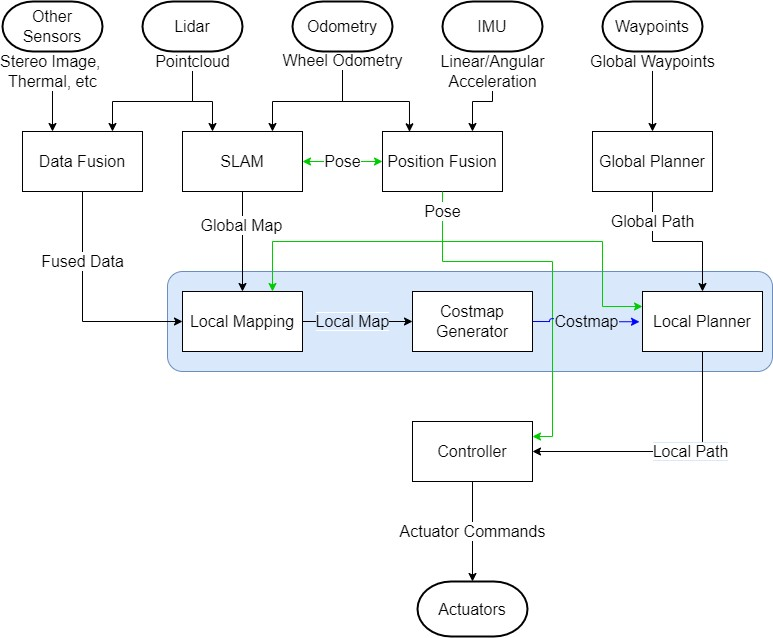
\includegraphics[width=0.85\textwidth]{figures/fig_ugv_system_overview}
    \caption{System overview of a typical unmanned ground vehicle.}
    \label{fig:ugv_system_overview}
\end{figure}

\section{Off-Road and Agricultural Autonomous Navigation}

\subsection{Challenges in Off-Road Environments}

Off-road environments inherently present a significantly more complex and dynamic challenge for autonomous navigation systems compared to highly regulated, structured urban settings \citep{Ref277}. These unstructured spaces are characterized by unpredictable macro-topographical variations, including severe slope gradients, uneven surface profiles, and a dense distribution of heterogeneous environmental obstacles \citep{Ref277}. Specifically, an autonomous vehicle must continuously perceive and negotiate a wide array of static and dynamic anomalies---such as large rocks, structural depressions, and dense field vegetation---that disrupt steady traction and clear path traversal \citep{Ref277}. Consequently, managing these irregular environmental profiles requires a transition toward advanced navigation architectures capable of dynamically interpreting multi-dimensional workspace geometries.

Traditional 2D path planning architectures are fundamentally unsuited for these rough topographies because they operate on a simplified planar representation of the environment that completely neglects the crucial vertical dimension \citep{Ref228}. This structural oversight routinely leads to the generation of global trajectories that are geometrically optimal in terms of horizontal distance but physically un-traversable, unsafe, or highly inefficient when projected onto uneven ground \citep{Ref228}. For example, a planar navigation routine lacks the spatial mapping capacity to detect overhead clearance obstacles positioned above its observation plane or may guide a vehicle across a steep incline that exceeds the platform's physical climbing capabilities, resulting in catastrophic structural collisions or complete vehicle immobilization \citep{Ref228}. Therefore, executing safe and efficient off-road navigation necessitates a robust mathematical understanding and direct integration of three-dimensional terrain characteristics into the core path planning process.

\begin{figure}[htbp]
    \centering
    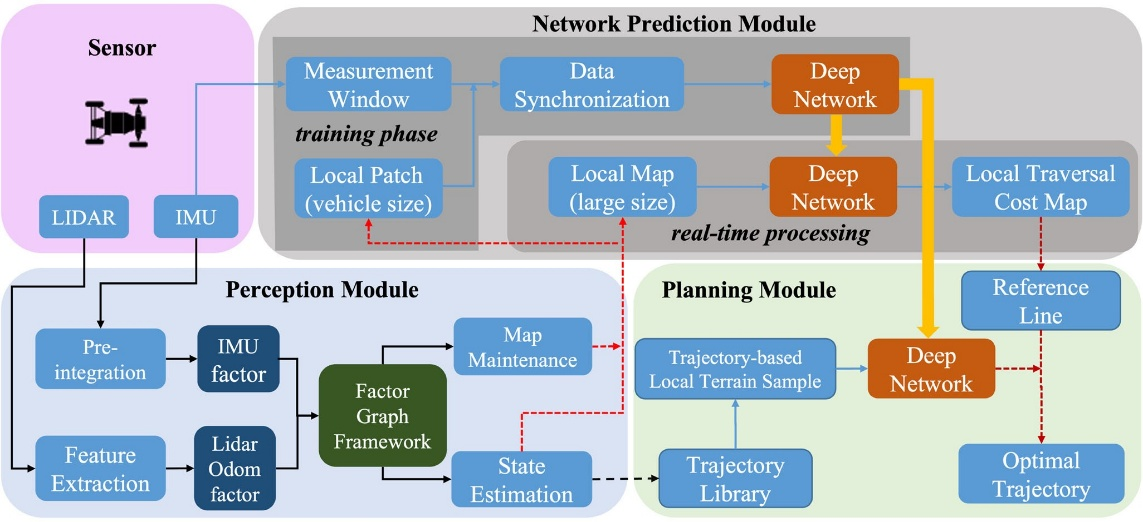
\includegraphics[width=0.85\textwidth]{figures/fig_nav_architecture}
    \caption{Architecture of the proposed autonomous navigation approach. During real-time navigation, the perception module provides the original point cloud map and the vehicle pose. The prediction module predicts the local point cloud map and performs traversal cost.}
    \label{fig:nav_architecture}
\end{figure}

\subsection{Autonomous Systems in Agriculture}

The ongoing integration of autonomous navigation technologies within the agricultural sector is primarily driven by expanding global food demands and an acute, long-term contraction of the skilled rural labor force \citep{Ref88}. To address these production bottlenecks, autonomous agricultural ground robots are increasingly being deployed across field operations to execute complex tasks such as precision seeding, automated harvesting, and broad-acre field surveillance \citep{Ref10, Ref14}. However, these unique field deployment scenarios impose rigorous and specialized architectural requirements on motion planning frameworks that extend far beyond standard urban navigation paradigms. Beyond simply achieving collision avoidance, agricultural mobile platforms must traverse complex crop layouts and undulating sloped landscapes both resource-efficiently and safely \citep{Ref10}. This multidimensional operational profile necessitates optimization across a diverse suite of competing performance criteria, including minimizing travel time constraints, reducing cumulative mechanical energy expenditure, and enforcing rigid platform stability on varying terrains to actively prevent catastrophic rollover accidents \citep{Ref10, Ref507}. Consequently, achieving high operational precision during in-field maneuvers underscores the vital importance of deploying terrain-aware path planning systems that explicitly account for localized topographic variations and variable surface conditions.

\subsection{Positioning Systems for Off-Road Vehicles}

Reliable three-dimensional (3D) navigation and deterministic path execution for autonomous off-road vehicles rely fundamentally on high-precision localization architectures. Modern state estimation suites typically fuse complementary sensor modalities to achieve robust, real-time vehicle positioning across unstructured terrains. For instance, Differential Global Positioning Systems (DGPS) provide absolute global coordinates, whereas Inertial Navigation Systems (INS) deliver high-frequency attitude rates and localized motion data \citep{Ref6}. The algorithmic integration of these asynchronous DGPS and INS measurements is commonly executed utilizing state-space architectures such as Extended Kalman Filters (EKF), which can be structurally deployed via either an error state space formulation or a total state space formulation \citep{Ref6}. While the total state space approach provides an optimally weighted blending of multi-sensor data profiles, its implementation introduces high computational iteration rates and increases systemic vulnerability to individual sensor failures \citep{Ref6}. These multi-sensor fusion frameworks significantly attenuate sensor noise and elevate the estimation accuracy of the vehicle's position, pitch, roll, and height configurations, which are critical for constructing high-fidelity environmental terrain maps and tracking planned global trajectories \citep{Ref6, Ref10}.

\section{Terrain Representation and Mapping for Off-Road Navigation}

\subsection{2D vs. 3D vs. 2.5D Terrain Models}

The selection of an optimal environmental mapping paradigm represents a critical design choice in off-road path planning, directly influencing an algorithm's computational complexity, geometric accuracy, and physical applicability. Traditional 2D grid maps simplify the workspace configuration into a flat plane, rendering global path generation highly efficient from a computational standpoint. Under this planar assumption, classical graph-search algorithms operate effectively within low-overhead tracking boundaries \citep{Ref45}. However, this flat abstraction is fundamentally limited when deployed across uneven or natural landscapes because it completely ignores crucial vertical geometry, routinely leading to the generation of physically untraversable paths, structural collisions, and catastrophic navigation errors \citep{Ref228}. Consequently, relying on flat surface assumptions strips the navigation system of its ability to proactively identify macro-topographical variations before path execution.

To overcome the spatial blindness of planar models, full 3D volumetric representations can be utilized to capture the complete, high-fidelity geometry of an unstructured environment. These multi-dimensional mapping frameworks preserve the complete spatial topology of the workspace, enabling comprehensive obstacle detection, negative obstacle mapping, and detailed traversability analysis. While ideal in theoretical formulations, full 3D representations introduce massive data densities and high geometric dimensionality that incur severe computational overhead \citep{Ref233}. This processing burden demands substantial runtime memory storage and processing power, making real-time path planning exceptionally challenging for computationally restricted embedded autonomous platforms \citep{Ref233}. As a result, the extreme processing latencies associated with dense volumetric data structures often limit their practical application in dynamic edge-computing scenarios.

Two-and-a-half-dimensional (2.5D) terrain models have emerged as a highly practical structural compromise, balancing the computational simplicity of 2D layouts with the rich geometric fidelity of full 3D configurations. This mapping paradigm correlates horizontal planar coordinates $(x, y)$ with a single, discrete altitude value $z$ for each individual grid cell, successfully preserving critical height variations and continuous surface characteristics \citep{Ref1, Ref2}. This coordinate abstraction allows pathfinding algorithms to execute direct, real-time evaluations of localized slope magnitudes (SM) and physical three-dimensional step distances (3DSD), which are critical for accurately quantifying traversability and calculating instantaneous movement costs \citep{Ref1, Ref228}. By integrating these vital vertical dimensions without inheriting full volumetric voxel densities, 2.5D configurations provide sufficient geometric detail for safe, resource-efficient off-road routing. This structural balance is particularly vital for autonomous agricultural vehicles, where executing stable navigation across sloped landscapes and unmanaged crop fields requires a highly nuanced, topologically aware understanding of terrain profiles to prevent platform instability \citep{Ref10}.

\begin{figure}[htbp]
    \centering
    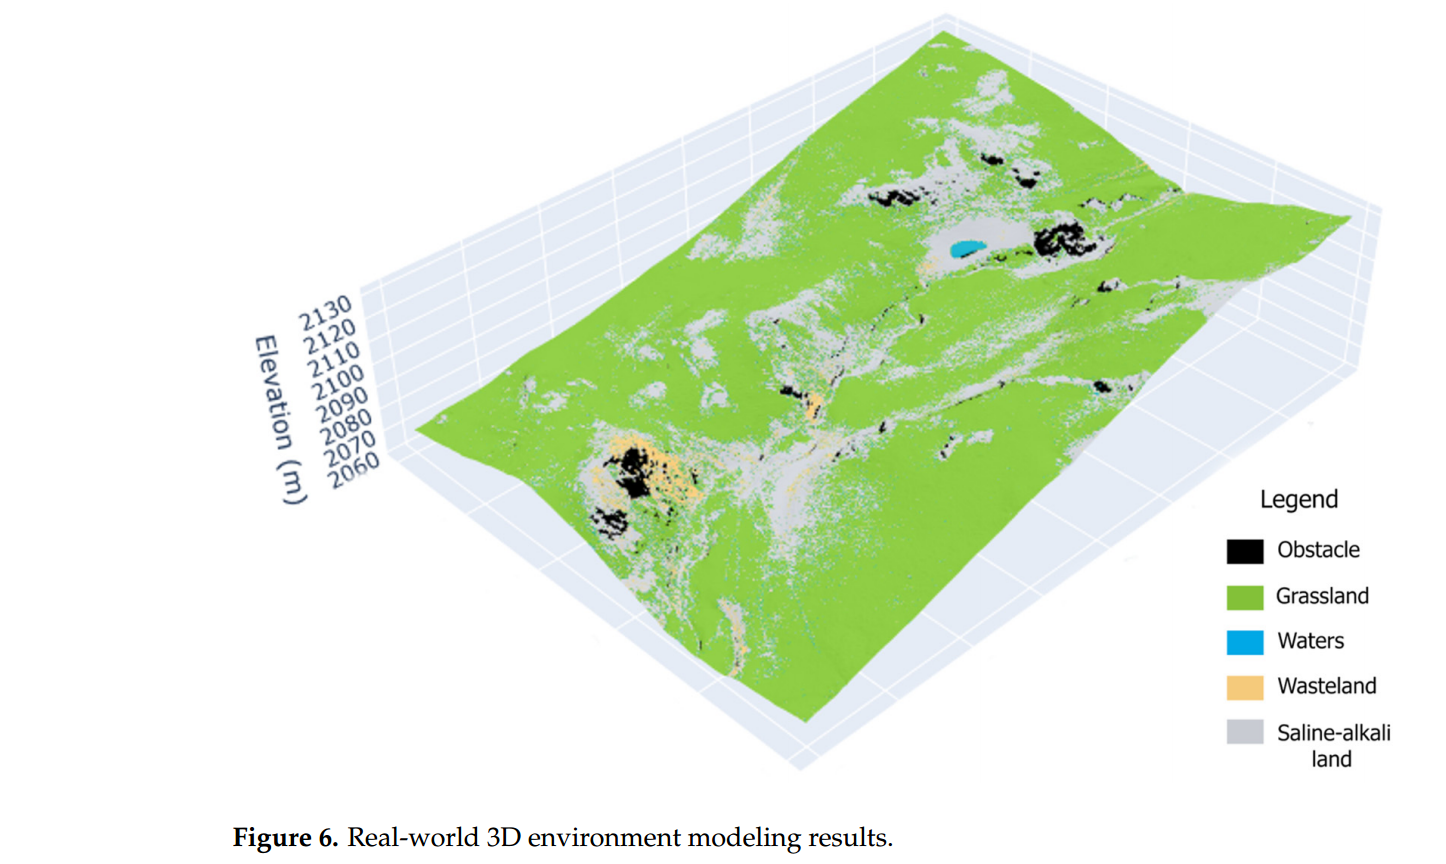
\includegraphics[width=0.85\textwidth]{figures/fig_3d_terrain_model}
    \caption{Real-world 3D environment modeling results.}
    \label{fig:3d_terrain_model}
\end{figure}

\subsection{Point Cloud Data and Grid-Based Mapping}

The systematic acquisition and processing of spatial environmental data represent the foundational phase in transforming raw, unstructured sensory inputs into actionable geometric matrices for mobile robot localization and path generation. This mapping pipeline predominantly begins with the collection of dense three-dimensional (3D) point cloud datasets, typically stored in .pcd file formats and captured via high-resolution Light Detection and Ranging (LiDAR) sensor suites \citep{Ref156}. To be utilized by global graph-search configurations, these unorganized spatial coordinate vectors must be mathematically parsed, filtered, and transformed into structured, low-overhead topologies, which for 2.5D terrain representations entails converting the volumetric points into a static elevation grid map \citep{Ref1}. This coordinate transformation is typically executed by discretizing a horizontal reference plane---such as the $XY$ plane---into a network of uniform square cells, and subsequently approximating the localized 3D environmental geometries and structural obstacles using discrete bounding cuboids parameterized by the minimum and maximum vertical coordinate values (e.g., the $Z$-axis) found within each grid boundary \citep{Ref1, Ref1}. Furthermore, spatially overlapping obstacles occupying a single cell coordinate are algebraically merged into a unified layer, establishing a definitive traversable domain bounded directly by the upper surface facets of these approximated bounding boxes \citep{Ref1}. This geometric projection technique compresses high-density volumetric point clouds into a streamlined, non-planar heightfield grid optimized for real-time pathfinding operations.

Beyond the mapping of rigid geometric macro-topographies, executing safe navigation within dense agricultural environments requires superimposing non-geometric semantic features onto the underlying spatial layout. To achieve this layered environmental awareness, the integration of a specialized single-layer vegetation penalty mask is necessary to model sections of the workspace that, while physically passable, introduce substantial locomotion resistance or risk inducing structural crop damage \citep{Ref156}. These non-binary cost layers operate by dynamically injecting scalar penalty values into coordinate cells that exhibit significant vegetation height or dense canopy distributions, thereby artificially inflating the local traversal cost during node expansion. By manipulating the heuristic search in this manner, the global path planner is proactively guided away from high-resistance, vegetative zones and steered toward cleaner, unencumbered paths. Layering these semantic cost metrics onto the baseline geometric elevation grid ensures that the generated trajectories respect both the hard kinematic limits of the terrain and the soft operational safety constraints of the agricultural environment.

\section{Path Planning Algorithms for Mobile Robots}

\subsection{Heuristic Search Algorithms (A* and its Variants)}

Heuristic search algorithms, particularly the A* algorithm, form the foundational bedrock of mobile robot path planning systems due to their proven mathematical optimality and operational efficiency within static environments \citep{Ref45, Ref101}. Mechanistically, the algorithm systematically explores a graph or a discretized grid network to compute a trajectory connecting an initial start node to a terminal goal state with the absolute minimum accumulative cost. To govern this deterministic graph search, A* implements a multi-variant evaluation function expressed as:

\begin{equation}
    f(n) = g(n) + h(n)
\end{equation}

\noindent where $g(n)$ represents the exact, accumulated cost traversed from the initial start node to the current node $n$ \citep{Ref45, Ref101, Ref279}. Concurrently, $h(n)$ acts as a heuristic function estimating the remaining traversal cost from node $n$ to the terminal goal state \citep{Ref45}. For the algorithm to preserve its mathematical guarantees of optimality and completeness, the design of $h(n)$ must remain strictly admissible---meaning it never overestimates the true remaining cost---and mathematically consistent \citep{Ref410}. This core cost infrastructure underpins the node selection strategy executed during live spatial exploration.

At an execution level, the graph search manages node categorization using two synchronized data structures known as the Open List and the Closed List \citep{Ref70, Ref126, Ref144, Ref181}. The algorithm operates through iterative optimization loops, continuously selecting the specific node that exhibits the lowest $f(n)$ value from the Open List, transitioning it to the Closed List, and evaluating its adjacent neighboring cells \citep{Ref70, Ref126}. To configure the structural topology of the grid network, implementing an 8-connected grid mapping paradigm permits both orthogonal and diagonal node transitions. This multi-directional connectivity offers superior spatial flexibility and generates significantly shorter path metrics than restrictive 4-connected grid allocations. The geometric behavior of these spatial transitions is directly tied to the mathematical distance equations selected for the heuristic estimator.

The localized search velocity and directional bias of the pathfinder are heavily governed by the specific spatial distance formula chosen to represent $h(n)$. For grid configurations where unconstrained multi-directional traversal is permitted, the Euclidean distance represents the absolute straight-line metric calculated as:

\begin{equation}
    h_{Euclidean}(n) = \sqrt{(x_{goal} - x_n)^2 + (y_{goal} - y_n)^2}
\end{equation}

\noindent which serves as a standard baseline across diverse pathfinding systems \citep{Ref45, Ref85, Ref279}. Alternatively, when vehicle translations are constrained to standard grid lines, the Manhattan distance maps orthogonal displacements via:

\begin{equation}
    h_{Manhattan}(n) = |x_{goal} - x_n| + |y_{goal} - y_n|
\end{equation}

\noindent which is optimal for restrictive grid layouts \citep{Ref45}. For grid environments that explicitly accommodate uniform diagonal movements along with orthogonal transitions, the Octile distance function computes the search space boundaries as:

\begin{equation}
    h_{Octile}(n) = \max(|x_{goal} - x_n|, |y_{goal} - y_n|) + (\sqrt{2} - 1) \cdot \min(|x_{goal} - x_n|, |y_{goal} - y_n|)
\end{equation}

\noindent which minimizes structural distance distortion \citep{Ref45}. Selecting the most structurally appropriate heuristic from these options is critical, as it directly shapes the algorithm's runtime efficiency and exploration footprint \citep{Ref410}.

Modern field robotics applications frequently require expanding these basic distance models into multi-objective frameworks to balance geometric length with environmental safety criteria. This expansion is typically achieved by altering the cost definition of $g(n)$ to explicitly penalize paths that threaten vehicle smoothness, compromise operational safety, or accelerate vehicle energy consumption \citep{Ref210, Ref309, Ref424}. For instance, in maritime routing domains, the core A* architecture has been improved to seamlessly integrate fluid water currents, traffic separation protocols, and localized maneuverability risks \citep{Ref85}. Similarly, off-road autonomous driving applications utilize modified graph-search models to evaluate instantaneous collision indices and rollover risks across dynamic environmental grid maps \citep{Ref507}. However, despite these advancements, the direct, real-time integration of three-dimensional step distances (3DSD) and localized slope magnitudes (SM) as intrinsic components of the cost function for 2.5D agricultural terrain planning, alongside a dedicated adjustable slope weight, remains an unresolved research gap.

To balance exploration breadth and goal-directed guidance during the node search, adaptive cost-weighting schemes are often incorporated into the core evaluation equations. A common linear weighting technique parameterizes the cost equation as:

\begin{equation}
    f(n) = g(n) + w \cdot h(n)
\end{equation}

\noindent allowing engineers to dynamically tune the trade-off between thorough search exploration ($w < 1$) and focused heuristic guidance ($w > 1$) \citep{Ref410}. Building upon this weighting concept, the framework developed in this thesis introduces an adjustable slope weight parameter ($\lambda$) designed to dynamically modulate the relative influence of topographic steepness within a unified multi-terrain cost structure. This approach contrasts sharply with kinematically constrained alternatives like the Hybrid A* algorithm, which couples discrete graph search with continuous motion primitives to guarantee drivable trajectories in constrained spaces \citep{Ref206}. While Hybrid A* effectively secures kinematic feasibility, its standard execution remains restricted to flat 2D occupancy grids, highlighting a lack of explicit, multi-dimensional terrain-cost integration.

\subsection{Other Path Planning Approaches}

While A* and its heuristic variations remain the algorithmic focal point of this research, alternative motion planning paradigms provide essential comparative context regarding multi-dimensional optimization. Sampling-based path planning algorithms, most notably Rapidly-exploring Random Trees (RRT) and Probabilistic Roadmaps (PRM), are highly effective when navigating high-dimensional or geometrically dense configuration spaces, offering mathematical guarantees of probabilistic completeness \citep{Ref380, Ref406}. Mechanistically, the standard RRT algorithm explores the vehicle's workspace by iteratively sampling random spatial coordinates and expanding a tree network from the nearest existing vertex toward these target samples \citep{Ref380, Ref452}. Concurrently, the PRM architecture constructs a continuous topological roadmap by validating interconnected networks of randomly distributed free-space samples and their visible local neighbors \citep{Ref406}. Although these sampling-based approaches effectively mitigate the ``curse of dimensionality'' that penalizes standard grid-allocation techniques, they introduce significant runtime memory overhead and require exhaustive iteration phases to converge toward true global optimality \citep{Ref406}. Consequently, their inherent stochasticity often yields structurally jagged trajectories that necessitate extensive post-processing smoothing to achieve physical execution.

Nature-inspired meta-heuristic algorithms represent an alternative class of global optimization techniques capable of approximating complex trajectories through stochastic search behaviors. Genetic Algorithms (GA), for example, iteratively evolve populations of candidate path solutions through selection, crossover, and mutation mechanisms, providing robust global search capabilities across non-linear spaces \citep{Ref417, Ref519}. These evolutionary mechanics can be combined with A* cost models to seed populations with high-quality heuristic profiles and accelerate structural convergence \citep{Ref284}. Similarly, Particle Swarm Optimization (PSO) maps candidate solutions as discrete particles moving through a multi-dimensional search space, where individual trajectories are guided by a weighted combination of personal historical optima and global swarm best-found states \citep{Ref266}. In agricultural routing, PSO frameworks have been implemented to generate real-time parametric paths that evaluate vehicle kinematic configurations alongside static terrain hazards \citep{Ref471}. Furthermore, Ant Colony Optimization (ACO) mimics swarm intelligence by deploying agents that collectively identify optimal routes via simulated pheromone deposition \citep{Ref368, Ref495}. Although ACO architectures require substantial computational iteration to reach steady-state convergence, optimized variants can dramatically improve processing throughput \citep{Ref368}. Despite their structural flexibility, the high computational overhead of meta-heuristics often restricts their applicability on resource-constrained embedded hardware.

To bridge global routing with real-time obstacle avoidance, local reactive windowing models are frequently fused with primary graph-search frameworks. The Dynamic Window Approach (DWA) is a popular local path planning algorithm that generates safe velocity commands for mobile robots in real-time by explicitly incorporating the platform's immediate mechanical and structural dynamics. The algorithm models the search space by sampling admissible acceleration profiles and evaluating short-horizon trajectories against a multi-variant objective function that scores target headings, obstacle clearance distances, and localized velocities \citep{Ref283, Ref396, Ref482}. By selecting the velocity command that maximizes this reactive function, DWA ensures that global paths adapt dynamically to localized changes without violating kinematic operating limits.

Alternatively, Artificial Potential Field (APF) methodologies model real-time navigation by treating the autonomous platform as a charged particle moving through a continuous virtual force field. Within this mathematical paradigm, the target destination generates an attractive potential gradient that pulls the vehicle forward, while local obstacles project a repulsive potential field that drives the vehicle away from structural hazards \citep{Ref266, Ref491}. While APF formulations are computationally inexpensive and highly optimized for instantaneous edge processing, they are systematically vulnerable to local minima traps where opposing forces cancel out, causing vehicle oscillations or complete path freeze-ups in cluttered environments \citep{Ref266, Ref491}. To mitigate these local minima vulnerabilities, hybrid architectures frequently couple APF forces with A* node selection loops to guide the vehicle out of dead-end configurations \citep{Ref152}. These reactive and force-based local planners provide the essential low-level velocity tracking necessary to physically execute optimized global paths.

\section{Trajectory Smoothing and Refinement}

\subsection{Need for Smoothing}

Global trajectories computed by discrete, grid-based search frameworks like the A* algorithm are fundamentally limited by their structural graph topology, which outputs a sequence of sharp, discontinuous waypoints that result in jagged or angular paths \citep{Ref45}. Executing these raw piece-wise linear path segments directly is highly undesirable for autonomous ground vehicles because they necessitate abrupt changes in the vehicle's heading vector. These rapid steering adjustments induce severe velocity tracking errors, high mechanical jerk, accelerated fatigue or wear across localized chassis components, elevated electrical power dissipation, and systemic tracking instabilities within low-level feedback controllers \citep{Ref45, Ref279, Ref470}. Therefore, implementing an algorithmic post-processing refinement step to transform these piece-wise discrete nodes into continuous, curvilinear trajectories represents a vital prerequisite for elevating vehicle drivability, minimizing tracking errors, and safeguarding platform structural integrity.

\begin{figure}[htbp]
    \centering
    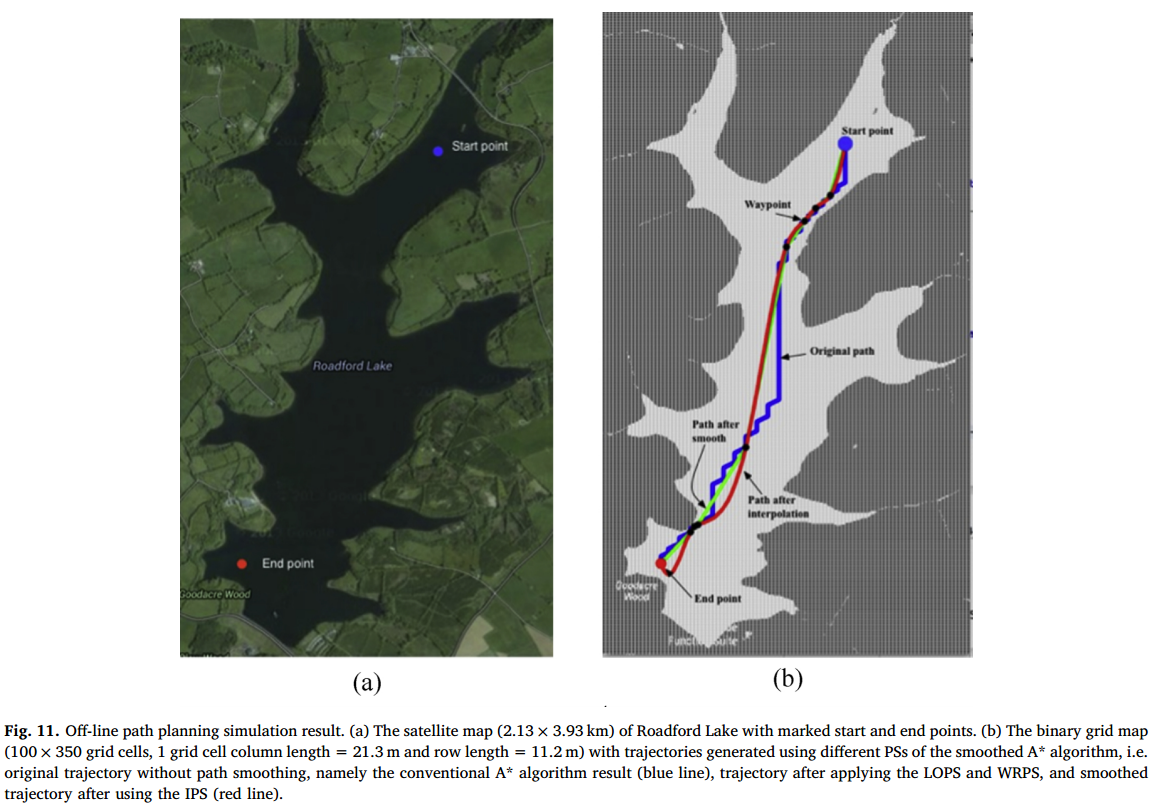
\includegraphics[width=0.85\textwidth]{figures/fig_chap3}
    \caption{Illustration of path smoothing applied to a discrete grid-based trajectory.}
    \label{fig:path_smoothing}
\end{figure}

\subsection{B-splines for Path Smoothing}

Among continuous parametric optimization formulations, B-spline curves have become a widely adopted method for trajectory smoothing due to their local support property and their ability to generate continuous, differentiable paths \citep{Ref279}. This mathematical formulation allows engineers to alter local curve shapes by manipulating discrete control point matrices without causing global geometric deformations, while simultaneously guaranteeing high-order parametric continuity across the trajectory profile \citep{Ref309}. Specifically, enforcing $C^2$ continuity---which mathematically secures continuous first and second derivatives---ensures that the vehicle's bounded lateral and linear accelerations remain smooth and uninterrupted during transit. To bound these parametric properties within defined global terminal states, utilizing open-uniform B-splines is advantageous because their clamped knot vectors force the continuous curve to pass exactly through the initial start and final goal nodes. Translating the discrete waypoints of the graph search into a structured control point matrix produces a kinematically feasible path that prevents sudden actuator saturation or physical freeze-ups during autonomous mobile robot execution \citep{Ref279}.

\subsection{Validation of Constraints during Smoothing}

Although geometric smoothing techniques enhance path aesthetics and velocity tracking performance, a critical research gap exists in rigorously coupling these continuous parametric refinements with concurrent validation of terrain-climbability thresholds and boundary constraints. Simply executing a curvature minimization routine can inadvertently alter the spatial coordinates of a path segment, shifting it onto hazardous topographies that violate the vehicle's hard physical limits, such as its Maximum Climbable Slope (MCS) \citep{Ref42}. Trajectories optimized without these physical considerations may appear visually fluid in the horizontal workspace but remain unsafe or impossible to traverse in non-planar settings \citep{Ref42}. Traditional path optimization frameworks typically restrict their safety evaluation loops to basic planar obstacle clearance and curvature smoothness criteria \citep{Ref45, Ref233}. However, robust off-road navigation architectures require the integration of continuous rollover hazard evaluations during path selection to guarantee platform stability over severe inclines \citep{Ref507}.

This thesis addresses these combined limitations by developing an integrated validation module that directly couples open-uniform B-spline refinement with a high-frequency discrete sampling check. This verification pipeline evaluates the continuous trajectory immediately following or during the curve optimization phase to ensure that the candidate path rigorously adheres to three key boundary parameters:

\begin{itemize}
    \item \textbf{Boundary Compliance:} Keeping the path within defined operational limits.
    \item \textbf{Vegetation Exposure:} Adhering to the limits of the vegetation penalty mask.
    \item \textbf{Maximum Slope Thresholds:} Ensuring no segment exceeds the vehicle's Maximum Climbable Slope (MCS) or other traversability limits.
\end{itemize}

Enforcing this multi-layered validation during post-processing is crucial for generating truly safe and traversable paths for autonomous off-road agricultural vehicles. Furthermore, data simplification techniques---such as the Douglas-Peucker algorithm or related collinear waypoint suppression methods---are frequently deployed prior to curve fitting to prune redundant nodes. This data reduction minimizes the computational load of the B-spline solver while preserving the underlying topological features of the path \citep{Ref102, Ref482}.

\section{Performance Metrics and Evaluation}

The comprehensive evaluation of path planning frameworks for autonomous off-road vehicles requires a multi-faceted approach, employing both standard and terrain-specific performance indicators to assess algorithmic utility. Relying solely on a single operational parameter provides an incomplete assessment of a navigation system's real-world viability. Consequently, modern field robotics literature establishes a verification paradigm that simultaneously benchmarks geometric accuracy, processing velocity, and kinematic feasibility. This multi-layered analytical lens is mandatory for quantifying the exact trade-offs introduced when augmenting a classical routing routine with multi-dimensional terrain awareness.

\subsection{Standard Performance Indicators}

The evaluation of global trajectory profiles begins with analyzing standard spatial and temporal parameters that govern the physical execution of a computed route. The most fundamental indicator is total path length ($L$), which reflects the geometric distance traversed by the vehicle from its starting configuration to the terminal goal state \citep{Ref29, Ref85, Ref309}. While conventional planar routines calculate this length over a flat projection, terrain-aware models must compute the true three-dimensional (3D) path length ($L_{3D}$) to account for vertical elevation variations along non-planar surfaces. Concurrently, algorithmic execution runtime and computational efficiency monitor the temporal processing load, logging the total time required to complete graph exploration, cost updates, and validation loops \citep{Ref54, Ref108, Ref169, Ref309, Ref424}. Securing minimized runtime latencies is paramount for ensuring edge-computing feasibility and enabling rapid trajectory adaptation to structural environmental changes. Finally, path smoothness metrics quantify the geometric curvature profiles and derivative continuity of the trajectory, directly influencing tracking stability, low-level actuator wear, vehicle ride comfort, and localized mechanical stress \citep{Ref45, Ref45, Ref309, Ref507}. Integrating dedicated steering penalties or post-processing B-spline refinement modules serves to systematically elevate this smoothness index, transforming jagged, node-based waypoints into kinematically executable curvilinear functions \citep{Ref45, Ref279}.

\subsection{Terrain-Specific Metrics (Proxies)}

Evaluating autonomous vehicle navigation across unstructured off-road and agricultural domains requires specialized performance metrics capable of quantifying the intricate physical interactions between a mobile platform and a non-planar terrain profile. Relying exclusively on classical geometric indices is insufficient for characterising cross-country mobility, as uniform horizontal displacements can exhibit wildly varying mechanical and temporal costs depending on the local slope gradient or soil configuration. Consequently, modern field robotics research relies on specialized mathematical proxies and physical threshold indices to evaluate a path's true operational viability before physical trajectory tracking.

The temporal efficiency of a non-planar route is evaluated using speed-adjusted travel-time proxies (TTP), which capture the localized velocity reductions that occur due to adverse terrain geometry and topography. While baseline navigation approaches frequently treat vehicle speed as a static, unvarying parameter \citep{Ref210}, advanced field robotics frameworks incorporate dynamic speed-reduction functions that scale velocity down based on severe slope inclinations, surface roughness, or localized obstacle proximity \citep{Ref440}. Concurrently, optimizing mechanical energy expenditure is a core requirement for ensuring long-endurance operations and economic viability in precision farming \citep{Ref10}. To model these thermal and fuel constraints without the complexity of full multi-body dynamics, architectures implement uphill-selective energy consumption proxies (ECP) within their evaluation loops \citep{Ref424}. These energy proxies operate by applying non-linear penalties to positive elevation changes along the path vectors, explicitly reflecting the heightened engine load and power draw required to overcome gravitational resistance during uphill climbs. Finally, an algorithm's fundamental safety and reliability are quantified via localized success rates and collision avoidance indices, which measure the statistical percentage of completed trials wherein the vehicle reaches its terminal goal state without encountering structural collisions or cross-country immobilization hazards \citep{Ref108, Ref253, Ref309}. In non-planar environments, this validation parameter focuses on assessing whether the trajectory remains bounded within localized regions that comply with the platform's hard physical Maximum Climbable Slope (MCS) limitations.

\subsection{Simulation Environments}

The utilization of virtual simulation environments represents a standard, highly effective methodological convention for prototyping, developing, and evaluating autonomous navigation architectures, particularly when confronting complex and hazardous off-road scenarios \citep{Ref108, Ref134, Ref154}. High-fidelity virtual simulations facilitate completely reproducible testing protocols across a diverse spectrum of heterogeneous terrain profiles---specifically low-gradient plains, medium-relief hills, and high-relief escarpments---under tightly controlled parameter distributions. This digital sandbox approach bypasses the severe logistical constraints, high capital costs, and physical safety hazards associated with real-world mobile platform deployments \citep{Ref214}. Open-source robotics middleware and simulators, most notably Gazebo, are widely used across the field robotics community to safely collect multi-sensor data collections, stress-test prediction networks, and validate global path planning behaviors prior to physical deployment \citep{Ref108}. Consequently, virtual benchmarking serves as a necessary and mathematically sound bridge between pure theoretical algorithmic modeling and physical field testing.

\section{Summary of Literature and Research Gap}

The contemporary body of literature establishes a robust technical foundation in traditional 2D and 3D path planning paradigms, with the classical A* graph-search algorithm serving as a structurally flexible and highly popular choice across diverse navigation sub-problems. The mathematical concept of 2.5D elevation maps is well-established as an effective structural compromise designed to balance rich geometric fidelity with minimized processing latencies in workspaces characterized by prominent vertical elevation changes \citep{Ref1, Ref228}. Furthermore, continuous parametric post-processing formulations, such as B-spline curves, are widely recognized for their mathematical capacity to transform piece-wise linear waypoints into smooth, differentiable, and kinematically suitable trajectories \citep{Ref279}. To quantify the efficacy of these integrated navigation systems, standard validation loops deploy a multi-faceted benchmarking suite that balances structural path lengths and execution runtime efficiency with qualitative criteria tracking curvature smoothness and vehicle collision safety \citep{Ref45, Ref45, Ref54}.

However, despite these foundational advancements, several critical technical gaps persist within contemporary literature, particularly concerning the terrain-aware navigation frameworks required for dynamic, complex agricultural off-road environments:

\begin{itemize}
    \item \textbf{Limited Integration of Comprehensive 3D Terrain Features in A* Cost Functions:} While specialized A* variants successfully incorporate isolated environmental modifiers---such as fluid water currents for maritime vessel routing \citep{Ref85} or general collision and rollover boundary risks for off-road driving \citep{Ref507}---the literature exhibits a clear absence of a unified, explicit cost function operating within a 2.5D A* configuration that simultaneously and directly evaluates physical three-dimensional step distances (3DSD) and localized slope magnitudes (SM). Crucially, the mathematical behavior and proactive path-hazard avoidance generated by combining these 2.5D terrain features with an adjustable slope weight parameter ($\lambda$) remains an unaddressed research contribution within the agricultural robotics domain.

    \item \textbf{Insufficient Validation of Constraints during Trajectory Smoothing:} Although continuous geometric refinement techniques like B-splines are widely applied to alleviate the sharp turning maneuvers output by grid-based planners, the consistent, rigorous coupling of these curve-fitting routines with concurrent terrain-climbability threshold enforcement and boundary constraint validation is not extensively addressed. This architectural gap means that smoothed paths that appear visually optimized may actually violate the platform's hard Maximum Climbable Slope (MCS) or stray outside defined workspace boundaries, leading to unsafe or impossible execution profiles.

    \item \textbf{Lack of Comprehensive Comparative Evaluations Against 2D Baselines:} While the implementation of diverse performance metrics remains standard convention for individual algorithm validation, the literature lacks a comprehensive, direct side-by-side comparative study contrasting a 2.5D terrain-aware A* implementation against a conventional flat 2D A* baseline across a spectrum of heterogeneous synthetic terrain profiles and adjustable slope weight ($\lambda$) configurations. This gap in empirical evaluation limits the quantified, mathematically grounded understanding of the specific operational advantages introduced by incorporating multi-dimensional terrain awareness into the core cost function.
\end{itemize}

This Master's thesis directly responds to these identified scholarly and engineering gaps through an integrated three-part research methodology. By formulating a 2.5D A* algorithm built upon a novel, unified multi-terrain cost function that simultaneously evaluates physical 3DSD, SM, and an adjustable $\lambda$, implementing a coupled B-spline smoothing and feasibility validation module, and conducting a comprehensive simulation-based comparative benchmark against a flat 2D baseline, this research delivers targeted, replicable solutions to each identified gap. The next chapter presents the detailed methodology developed to achieve these research objectives.
